\documentclass[12pt]{article}
%\usepackage{caption}
\usepackage{setspace,graphicx,epstopdf,amsmath,amsfonts,amssymb,amsthm}
\usepackage{marginnote,datetime,enumitem,subfigure,rotating,fancyvrb}
\usepackage{hyperref,float}
\usepackage[longnamesfirst]{natbib}
\usepackage{mathtools}
\usepackage{caption}
\usepackage{float}
\usepackage{lscape}
\usepackage{graphicx}
\usepackage{flafter} 
\usepackage{tabularx} 
\usepackage{booktabs}
\usepackage{changepage}
\usepackage{setspace}
\usepackage{placeins}
\usepackage{threeparttable}
\usepackage{ragged2e}
\usepackage[export]{adjustbox}
\newcolumntype{Y}{>{\raggedleft\arraybackslash}X}% raggedleft column X
\usdate
\usepackage[a4paper,bindingoffset=0.2in,%
            left=1.1in,right=0.85in,top=1in,bottom=1in,%
            footskip=.25in]{geometry}


% SCRIPTS:
% used SP19_rm_27 to create all the tables with monthly returns

% Number paragraphs and subparagraphs and include them in TOC
\setcounter{tocdepth}{2}

% JF-specific includes:

\usepackage{indentfirst} % Indent first sentence of a new section.
\usepackage{endnotes}    % Use endnotes instead of footnotes


\begin{document}

\setlist{noitemsep}  % Reduce space between list items (itemize, enumerate, etc.)
\onehalfspacing      % Use 1.5 spacing
% Use endnotes instead of footnotes - redefine \footnote command
\renewcommand{\footnote}{\endnote}  % Endnotes instead of footnotes

\author{Mykola Pinchuk\thanks{\rm Simon Business School, University of Rochester. Email: Mykola.Pinchuk@ur.rochester.edu. \newline I would like to thank Alan Moreira, Shuaiyu Chen, Xuyanda Qi and David Swanson for helpful comments.}}

\title{\Large \bf Cross-Industry Dispersion and Expected Retruns}

\date{10 September 2019}             % Final submission before Oct. 15

% Create title page with no page number

\maketitle
\thispagestyle{empty}

\bigskip

%\normalsize

\centerline{\bf ABSTRACT}

\small
\begin{onehalfspace}  % Double-space the abstract and don't indent it
  \noindent This paper examines cross-industry dispersion (CID), defined as a mean absolute deviation of returns of 49 industry portfolios. I find that expected stock returns are related cross-sectionally to the sensitivities of returns to innovations in CID. Annualized returns of the stocks with high sensitivity to CID are 8.4\% lower than the returns of the stocks with low sensitivity. This return spread is not explained by common factors, since abnormal returns with respect to the best factor model exceed 6\%. CID predicts unemployment, consistent with the hypothesis that CID is a proxy for unemployment risk due to sectoral shifts.
\end{onehalfspace}
\normalsize
\medskip


\clearpage
%\doublespacing
\setstretch{1.6}


\section{Introduction} \label{sec:Model}
Economy is a dynamic system with permanently evolving structure. As some industries are born, the other industries are losing their importance. A few people in 1970s could have predicted that within 20 years IT sector would capture the largest share of the stock market. There is no reason to expect a constant rate of this structural transformation. Naturally, accelerated structural transformation increases aggregate economic uncertainty and labor income risk for workers in underperforming industries. This paper explores asset pricing implications of such structural uncertainty.
\paragraph{}
I document a novel evidence that stock exposures to cross-industry dispersion (CID) predict cross section of expected returns. CID is defined as a mean absolute deviation of the returns of 49 industry portfolios. The paper finds that the firms with large return sensitivity to CID deliver smaller returns than the stocks with low sensitivity to CID. This finding suggests that in equilibrium there exists an extra demand for stocks, positively comoving with CID, implying low expected returns of these stocks. Long-short value-weighted portfolio, formed on the sensitivity to CID, delivers monthly return of 70 bps with abnormal returns of 50-80 bps. The results are not explained by the other measures of volatility and uncertainty.
\paragraph{}
This evidence is consistent with several sources of risk, possibly related to CID. Periods of highly nonhomogeneous performance of different industries (high CID) are likely to be the periods of increased economic uncertainty. Times of large wedge between winning and losing industries can proxy for the periods of rapid economic transformation, when some industries become more important, while the others lose relevance. During these periods investors are likely to have less understanding of the economic environment, reflecting growing uncertainty. Moreover, economy is more vulnerable to shocks within such uncertain times. Alternatively, high CID may indicate temporary decrease in output and efficiency as resources are reallocated across sectors (Lilien 1982). Since risk-averse agents lose utility when uncertainty rises, they create hedging demand for the stocks, whose returns positively comove with CID.
\paragraph{}
Labor income risk is another possible channel, explaining relevance of CID to asset pricing. By construction, high CID means that some industries severely underperform the market, while the others enjoy exceptionally high returns. This pattern is likely to raise a concern that losing industry is under the threat of dying. Naturally, this is a period of a negative shock to expected lifetime labor income of the employees in underperforming industries. The fact that there are both outperforming and underperforming industries with returns sufficiently far from the market return implies even larger labor income risk that the one during the recession. Within the recession, the common wisdom is that most of lost jobs will be recovered at some point in the future, while a disappearance of some industry means a loss of the jobs forever. 
\paragraph{}
While many occupations are demanded across industries, they are usually low skill occupations, less relevant to asset pricing. Losing high-wage job constitutes larger negative shock to lifetime income. Moreover, high-paid workers are likely to have more savings and produce larger effect on financial market. High-skill jobs (e.g., aerospace engineer) are usually confined to a few industries, implying very low across-industry labor mobility. Thus, I expect that CID captures asset pricing effect of Cross-sectional Dispersion (CSD), consistent with labor income risk. According to labor income risk explanation, stocks with negative covariance with CID are more risky, since they tend to fall when the risk of losing high skill industry-immobile jobs is large.
\paragraph{}
This paper draws upon the theoretical contribution of Duffie and Constantinides (1996) to motivate CIV as a state variable. Duffie and Constantinides show that in the model with heterogeneous agents, subject to uninsurable labor income shocks, cross-sectional variance of agents` consumption growth becomes a state variable. As discussed above, severe underperformance of their industry suggests a negative shock to expected consumption growth of employees.
\paragraph{}
This article builds upon a body of macroeconomic literature. Lilien (1982) reports that sectoral shifts and performance dispersion result in unemployment shocks, caused by migration of employees between firms and sectors. Loungani, Rush and Tave (1990) construct stock market dispersion index and document that it predicts unemployment. Brainard and Cutler (1993) use similar measure to assess the contribution of sectoral reallocation to unemployment. They find that sectoral reallocation accounts for a large share of unemployment fluctuations at long horizons. Multiple studies (Summers and Carrol 1991, Blundell, Pistaferri and Preston 2008, Guvenen and Smith 2014) document that households do not completely insure their consumption from persistent shocks to their labor income. These findings highlight the importance of labor income risk for asset pricing.
% lrt90 and bc93 used exactly the same cid and got the results. it seems that i already have at least some weak positive results, consistent with my labor story.
\paragraph{}
The research on economic uncertainty frequently uses cross-sectional dispersion of accounting variables as a measure of uncertainty. Bloom (2009) documents strong correlation between time-series measures of market volatility, cross-sectional variation of firms` pretax profit growth and returns as well as a dispersion across macroeconomic forecasts. He argues that all of these variables proxy for financial and macroeconomic uncertainty. Sadka (2012) finds that higher earnings dispersion is associated with higher expected returns, suggesting that earnings dispersion is a state variable, relevant for asset pricing.
\paragraph{}
This study contributes to several domains of literature. Different measures of market volatility have traditionally been used as a proxy for economic and financial uncertainty. Ang et al (2006) empirically show that exposure of stocks to VIX is priced in cross-section of expected stock returns. Kelly et al (2016) report that stocks with larger sensitivity to common idiosyncratic volatility (CIV) earn lower expected returns. They argue that CIV proxies for idiosyncratic risk faced by households and suggest labor income risk as a main channel.
\paragraph{}
This paper is closely related to the literature on cross-sectional dispersion (CSD), defined as a standard (mean absolute) deviation of the cross section of stock returns. Bekaert and Harvey (1997, 2000) use CSD as a measure of a development and a maturity of the stock market. Stivers (2003, 2006, 2010) finds that CSD can predict idiosyncratic volatility as well as returns of value and momentum premia. Maio (2013, 2016) reports that cross-sectional standard deviation of returns of the portfolios, sorted on size and book-to-market can predict market returns. The closest paper to this one is Verousis and Voukelatos (2018). It finds that the stocks with high sensitivity to CSD offer lower returns in the 1996-2012 sample. Due to more idiosyncratic nature of CSD, the authors explain the findings by idiosyncratic risk without elaborating on or providing evidence for this explanation.
\paragraph{}
This paper uses 1963-2018 sample and shows that high sensitivities to CID predict lower expected returns. I argue that this predictability stems from return dispersion across industries, proxying for labor income risk due to sectoral shifts. The results suggest that only across-industry component of CSD (i.e., CID) is priced. Long-short portfolio, formed on CID, controlling for CSD, delivers 32 bps (t-statistic=2.46) in monthly returns, while long-short portfolio, formed on CSD, controlling for CID, produces -3 bps returns. Therefore, the results suggest that cross-sectional predictability of returns by CSD is not driven by idiosyncratic risk, relevant for underdiverisified investors. CSD is a manifestation of more fundamental economic force - labor income risk due to structural shifts, proxied by CID. Consistent with this explanation, CID predicts future unemployment. To provide stronger evidence for this hypothesis, I intend to perform formal tests of this hypothesis in the next version of the paper using occupation-level employment data.
% there was the paper Jiang(2010), which seems totally retarded to me. the guy found 26% annualized quintile spread using beta from regression of returns on levels and explained it with the risk story with the wrong sign. do not want to cite it %.


\section{Data and Dispersion Measures} \label{sec:Model}

\subsection{Sample}

The paper uses stock price data from CRSP and accounting data from Compustat. The sample encompasses 1963-2018. I download macroeconomic data from St. Louis Federal Reserve Bank. 
I consider common stocks traded at NYSE, NASDAQ or AMEX and perform the main asset pricing tests at monthly frequency. The sample of stock returns consists of 3107556 firm-month observations with nonmissing returns. In order to exclude small and illiquid stocks from the analysis, I restrict the sample to the stocks with stock price above \$10 and the stocks with market capitalization above \$10 million in 2018 dollars. After this restriction the sample consists of 1741865 firm-month observations. All the analysis below uses excess returns.
\paragraph{}
I obtain the data on stocks market factors from Kenneth French`s website. I download uncertainty indices, constructed by Ludvigson et al. (2015) from Sydney Ludvigson`s website. Industry classifications as well as returns of industry portfolios are taken from Kenneth French`s website. 

\subsection{Construction of Dispersion Measures}

The paper defines cross-industry dispersion as a mean absolute deviation of returns across 49 industry portfolios at any given period. 
$$CID_t = \frac{1}{N}\sum^{N}_{i=1}{|R_{it}-R_{MKT,t}|}.$$
I use daily value-weighted returns of Fama-French 49 industry portfolios. I compute CID every day during the period 1927-2018. Since some industries have few firms at the beginning of the sample, the paper computes CID across the industries with at least 10 firms. I proxy by market return with value-weighted market return across all firms from CRSP (vwretd variable). I use the similar approach to calculate Cross-Sectional Dispersion (CSD) and Within-Industry Dispersion (WID).
\paragraph{}
The Figure 1 plots time series of CID. Since the paper follows asset pricing literature and starts the sample of stock returns in 1963, I focus on CID after 1963. Time series of CID exhibits two large secular increases. The first long-term spike took place within 1998-2003 and is likely to be associated with dotcom boom and the following decline. The second spike was recorded during 2007-2009, coinciding with the recent financial crisis. Both events are consistent with the hypothesis that CID proxies for some dimension of uncertainty and is related to the rate of sectoral shifts in the economy. Intuitively, CSD is a sum of CID and WID, so Figure 1 facilitates comparison of these variables. While before 2000, CSD was primarily driven by WID, during recent two decades CID and WID appear to contribute equally to CSD. This observation suggests increased comovement of returns within industries and a growing importance of a classification of firms into industries.
\paragraph{}
The next step of the analysis will be to estimate sensitivities of the stocks to fluctuations in CID. To facilitate interpretation of CID as a state variable from ICAPM and avoid econometric issues, I difference CID, using the same specification as in Pastor and Stambaugh (2003). That is, I calculate first differences of CID and estimate its residuals from AR(1) model:
$$\Delta(CID_t) = \gamma_0 + \gamma_1 \Delta(CID_{t-1}) + \gamma_2 CID_{t-1} + u_t.$$
Abusing notation, I refer to the residual $\hat{u}_t$ as $CID_t$ in the rest of the paper. 1-lag autocorrelation of CID is -0.07, implying very low persistence. Thus, I can use $CID_t$ as an explanatory variable in predictive regressions without spurious regression issues. 
\paragraph{}
Table 1 reports correlations of CID with other measures of uncertainty and volatility. Since all time series are differenced according to Pastor and Stambaugh (2003) specification, the correlations are relatively low. CID has positive correlation with all the variables, ranging from 0.09 to 0.3. The results suggest that CID is distinct from, though positively related to frequently used uncertainty and volatility measures.

\section{Asset Pricing Results} \label{sec:Model}

This section documents and discusses the main results of the paper. First, I explain how I estimate the sensitivity of stocks returns to CID. Then, I form decile portfolios on $\beta_{CID}$ and compute their returns. Finally, the section discusses asset pricing performance of different measures of cross-sectional dispersion.

\subsection{Estimation of $\beta_{CID}$}
I use daily stocks returns in order to obtain precise estimates of their sensitivities to CID. The paper uses two years of daily excess returns to estimate betas from the following regression:
$$R_{it}=\alpha+\beta CID_t + \epsilon_t.$$
Since controlling for market returns have little effect on the results, I use simpler specification. I estimate betas over the period 1963-2018. To compensate for extreme values of $\hat{\beta}_{CID}$, possibly resulting from imprecise estimation, I winsorize $\hat{\beta_{CID}}$ at 1\% and 99\% percentiles. 

\subsection{Portfolios, formed on $\beta_{CID}$}

In the remainder of this section, the paper uses monthly frequency. Every month, I sort the stocks into decile portfolios based on their $\beta_{CID}$. I update estimates of $\beta_{CID}$ and rebalance portfolios every month. To calculate postranking betas, I run the  regression above for each decile portfolio. Figure 2 plots post-ranking betas against pre-ranking betas. Not surprisingly, the spread decreases from 3 in pre-ranking betas to 0.6 in post-ranking betas. Clearly monotonic and almost linear relationship between post-rang and pre-ranking betas suggest that pre-ranking betas are reasonably good estimates of post-ranking betas. 
\paragraph{}
Table 2 reports mean values of characteristics of decile $\beta_{CID}$-sorted value-weighted portfolios. Stocks in the highest decile are usually larger, more profitable, more liquid, have slower asset growth and low past returns. Table 3 describe excess returns of equally-weighted and value-weighted portfolios, formed on $\beta_{CID}$. Equally-weighted long-short portfolio has average returns of 89 bps, though this spread is mostly driven by the returns of the first decile. Returns of value-weighted portfolios, sorted on $\beta_{CID}$, decrease almost monotonically. Long-short value-weighted portfolio generates 70 bps in average monthly returns with t-statistic of 3.9. 
\paragraph{}
Table 4 presents abnormal returns of value-weighted decile portfolio with respect to most frequently used factor models. Controlling for Fama-French 5 factors does not have significant effect on the returns of this trading strategy. T-statistics of these abnormal returns stays comfortably above 3, meeting the challenge of Harvey et al. (2016). Fama-French 5 factor model, augmented with momentum and short-term reversal factors, somewhat decreases abnormal returns to 50 bps (t-statistics = -2.9). While the loadings on size, momentum and short-term reversal factors can explain a fraction of the returns of this trading strategy, the loadings on market and value factors make this returns even more anomalous (Table 5).
\paragraph{}
Table 6 reports the returns of long-short portfolios, double-sorted on size and CID. Even controlling for size, long-short portfolio from tercile sorts on CID deliver statistically significant abnormal returns of 22-31 bps. Controlling for momentum factor decreases the returns to 15-16 bps. The weaker results are likely driven by both size factor and low precision of $\beta_{CID}$ estimates, combined with very coarse sorts.

\subsection{Cross-sectional Results}

To check a robustness of cross-sectional predictability of returns by $\beta_{CID}$, I employ Fama-MacBeth regressions. Table 7 reports that $\beta_{CID}$ is a significant determinant of excess returns (t-statistic above 2.4). Consistent with the previous findings, the results weaken after controlling for a size. An increase in $\beta_{CID}$ by 1 unit is related to 1.13\% lower excess returns. Since standard deviation of $\beta_{CID}$ is 1.00, the results suggest that 1 standard deviation increase in $\beta_{CID}$ is associated with 1.13\% smaller returns. Therefore, estimated price of CID risk is 1.13\%. Small economic magnitude of this number can be a result of the estimation, based on linear regression, capturing only linear relationship. Nonparametric results above suggest larger magnitude of CID risk premium.

\subsection{Performance of different dispersion measures}

Verousis and Voukelatos (2018) find that in 1996-2012 sample lower CSD is associated with high excess returns. The obvious question is whether asset pricing relevance of CSD is driven by its across-industry component (CID) or within-industry component (WID). To answer this question, I perform double sorts on WID and CID. Table 8 reports the results with value-weighted portfolios from 5x5 double sorts. I construct the long-short portfolio from the sort on CID, controlling for WID and vice versa. The long-short portfolio from WID sorts delivers abnormal returns between 22 and -19 bps, significantly different from zero. The long-short portfolio from CID sorts produces abnormal returns between 34 and 59 bps, which are highly significant. This results clearly imply that unlike WID, CID captures asset pricing-relevant dimension of cross-sectional dispersion. 
\paragraph{}
Table 9 reports the similar results from 5x5 double sorts on $\beta_{CID}$ and $\beta_{CSD}$. Long-short portfolio from CSD sorts produces significantly negative abnormal returns with respect to Fama-French 5 factor model, augmented with momentum factors. Since these returns have the sign, inconsistent with idiosyncratic risk explanation of Verousis and Voukelatos, the results clearly suggest that CSD predicts cross section of expected returns only through CID. Controlling for CSD, CID long-short portfolio generate abnormal returns between 26 and 43 bps with t-statistics above 2. Overall, the results suggest that CID reflects priced component of cross-sectional volatility.

\section{Economic Channel: Labor Income Risk} \label{sec:Model}

\subsection{Economic Mechanism and Hypotheses}

Constantinides and Duffie (1996) develop the model with agents, subject to heterogeneous uninsurable income shocks. They show that cross-sectional variance of individual consumption growth enters Euler equation. While the model analytically proves the relevance of cross-sectional consumption growth for asset pricing, it remains silent on its economic channels and meaning. This story naturally fits macrolabor literature which uses different measures of dispersion of stock returns to assess unemployment shocks, resulting from structural shifts.
\paragraph{}
Fluctuations in individual labor income can arise from two channels: change in wage and change in employment. Larger magnitude of labor income shocks from employment loss as well as downward wage rigidity suggest that unemployment risk is the most important component of labor income fluctuations for asset pricing. Macroeconomic literature views the changes in aggregate employment as the result of two forces: aggregate shocks and reallocation shocks. Lilien (1982) introduces sectoral shifts hypothesis entailing that higher dispersion of intersectoral shifts leads to higher unemployment by increasing amount of labor reallocation. While Lilien uses the variance of employment growth across sectors to measure the reallocation, Loungani, Rush and Tave (1990) argue that variance of stocks returns across sectors is more precise and forward-looking measure. 
\paragraph{}
This paper uses CID to capture a divergence in the performance across industries, indicative of a change in sectoral composition of the economy. Therefore, periods of high CID are indicators of increased risk of losing lobs in underperforming industries. While many occupations are not industry-specific (e.g., janitor), the others are closely related to a few industries (e.g., aerospace engineer). Potential disappearance of underperforming industry constitutes large labor income risk for such high-skill industry-specific occupations. \paragraph{}
The aggregate risk of unemployment due to sectoral shifts is larger when:
\begin{enumerate}
    \item {The threatened industry has more jobs.}
    \item {The threatened industry has large fraction of industry-specific jobs.}
    \item {The threatened industry consistently underperform other sectors.}
\end{enumerate}
This implications allow to modify the construction of CID to better capture the nature of unemployment risk from sectoral shifts. Therefore, I can test labor income explanation of CID premium by testing the following hypotheses:
\paragraph{}
\textbf{Hypothesis 1}: The abnormal returns of trading strategy, formed on $\beta_{CID}$ (i.e., CID premium) are larger when the underperforming industry has more employees.
\paragraph{}
\textbf{Test 1a}: The abnormal returns of trading strategy, formed on $\beta_{CID}$ are smaller then those of the trading strategy, formed on $\beta_{EWDCID}$, where $EWDCID=$.
\\ \-\hspace{0.3cm}
\textbf{Test 1b}: $R^{LS}_{t} = \gamma_0 +\gamma_1 Employment_{t-1}+\epsilon_t$. \\ 
According to Hypothesis 1, $\gamma_1>0$.
\paragraph{}
\textbf{Hypothesis 2}: The abnormal returns of trading strategy, formed on $\beta_{CID}$ are larger when the underperforming industry has larger fraction of high-skill workers.
\paragraph{}
\textbf{Test 2a}: The abnormal returns of trading strategy, formed on $\beta_{CID}$ are smaller then those of the trading strategy, formed on $\beta_{HWDCID}$, where $HWDCID=$.
\\ \-\hspace{0.3cm}
\textbf{Test 2b}: $R^{LS}_{t} = \gamma_0 +\gamma_1 HighSkill_{t-1}+\epsilon_t$. \\ 
According to Hypothesis 2, $\gamma_1>0$.
\paragraph{}
\textbf{Hypothesis 3}: The abnormal returns of trading strategy, formed on $\beta_{CID}$ are larger when the underperforming industry has lower returns during the past year.
\paragraph{}
\textbf{Test 3a}: The abnormal returns of trading strategy, formed on $\beta_{CID}$ are smaller then those of the trading strategy, formed on $\beta_{PWDCID}$, where $PWDCID=$.
\\ \-\hspace{0.3cm}
\textbf{Test 3b}: $R^{LS}_{t} = \gamma_0 +\gamma_1 PastReturns_{t-1}+\epsilon_t$. \\ 
According to Hypothesis 3, $\gamma_1>0$.
\paragraph{}
\textbf{Hypothesis 4}: The abnormal returns of trading strategy, formed on $\beta_{CID}$ are larger when the underperforming industry lost more employees during the past year.
\paragraph{}
\textbf{Test 4a}: The abnormal returns of trading strategy, formed on $\beta_{CID}$ are smaller then those of the trading strategy, formed on $\beta_{LEWDCID}$, where $LEWDCID=$.
\\ \-\hspace{0.3cm}
\textbf{Test 4b}: $R^{LS}_{t} = \gamma_0 +\gamma_1 LostEmployees_{t-1}+\epsilon_t$. \\ 
According to Hypothesis 4, $\gamma_1>0$.
\paragraph{}
Since identification of industry-specific jobs can be a challenging task, Hypothesis 2 proxies for them by high-skill jobs. 

\subsection{Results and future work}

Table 11 shows that CID predicts unemployment at quarterly frequency, controlling for other stock market-based predictors of business cycles. These results are consistent with findings of Loungani, Rush, Tave (1990) and Brainard, Cutler (1993) and suggest that CID can forecast unemployment shocks. While this evidence is consistent with CID proxying for labor income risk in a broad sense, it is silent on the nature of this unemployment shocks.
\paragraph{}
To provide the evidence on the relationship between CID and unemployment risk due to sectoral shifts, I intend to check whether CID predicts dispersion in employment growth across sectors.
\paragraph{}
In order to formally test the explanation of the trading strategy by unemployment risk due to sectoral shifts, I plan to perform Tests 1-4. I intend to use BLS OEM (Occupational Employment Statistics) dataset, containing information on statewide employment across occupations and industries at annual frequency. 
\paragraph{}
Since suggested economic channel hinges upon labor market mobility across industries, using product market-based industry definitions is somewhat arbitrary. I plan to explore OEM data and possibly construct occupation-based industry definitions.


\section{Further results} \label{sec:Model}
\subsection{Robustness to different industry definitions}

Since Fama-French (FF) 49 industry classification is arbitrary, I explore the robustness of the findings to industry definitions at the varying levels of coarseness. I compute CID using FF30, FF17, FF10 and FF5 definitions. Figure 4 reports CID premium at the different levels of industry aggregation. The results change a little as industry coarseness increases. Surprisingly, we observe large CID premium even as the paper computes CID from 5 industry portfolios. The results suggest that CID premium reflect the variation of returns between few broad industries.  
\paragraph{}
Fama-French industry classification is based on product market, so it is not a perfect measure for CID premium, hypothetically driven by labor income risk. Therefore in the later versions of the paper I will attempt to use/construct industry classifications, based on labor market competition and a type of workers` human capital. 

\subsection{Robustness to other uncertainty measures}

Table 1 reports the correlations between CID and other measures of uncertainty: VIX, market volatility, financial uncertainty (Ludvigson 2015), macroeconomic uncertainty (Ludvigson 2015) and common idiosyncratic volatility (Kelly 2016). Consistent with the hypothesis that all these variables capture financial uncertainty, CID has a positive correlations with all of them. On the other hand, the largest correlation of CID with these variables is 30\%, implying that CID is not a noisy proxy for these uncertainty measures.
\paragraph{}
Table 10 reports the relationship between CID premium and aforementioned uncertainty variables. I use 5x5 double sorts to control for sensitivities to these uncertainty measures. Double sorts on $\beta_{CID}$ and $\beta_{Vol}$ indicate that both variables deliver large risk premium, robust to controlling for asset pricing factors. Long-short portfolio, constructed on $\beta_{CID}$ sorts, produces abnormal returns between 30 and 48 bps and t-statistics above 2.48. Panels C and D show that $\beta_{CID}$ subsumes the relationship between stock sensitivities to financial and macroeconomic uncertainty (Ludvigson 2015) and expected returns. 
% need to read that paper, because i am not sure that they claim that.
The Panel B suggests that $\beta_{CID}$ outperforms $\beta_{CIV}$. Abnormal returns of $\beta_{CID}$-based long-short portfolios range between 26 and 44 bps versus 8 and 27 bps for $\beta_{CIV}$-based long-short portfolio. $\beta_{VIX}$ is the only variable, controlling for which eliminates statistical significance of CID premium. Controlling for VIX exposure, long-short portfolios, formed on $\beta_{CID}$, deliver 15-38 bps abnormal returns. Since these returns are economically significant and a loss of statistical significance appears to be driven by less precise estimates, I would hesitate to say that VIX exposure explains CID premium.

\subsection{Results at lower frequency}



\newpage

\section{Conclusion} \label{sec:Model}

This paper introduces CID as a measure of labor income risk due to sectoral shifts and explores its asset pricing implications. Stocks with low sensitivity to $\beta_{CID}$ are more risky, since they decline precisely when investors are subject to increased labor income risk. Consistent with this notion, these stocks produce higher returns. Value-weighted long-short portfolio, formed on $\beta_{CID}$, delivers 70 bps monthly returns. Abnormal returns range between 50 and 80 bps. The results are not explained by known measures of uncertainty and labor income risk, such as VIX (Ang et al. 2006), macroecocnomic and financial uncertainty (Ludvigson et al 2015) or common idiosyncratic volatility (Kelly et al. 2016). I show that previously documented cross-sectional predictability of returns by cross-sectional dispersion (Verousis and Voukelatos 2018) is a manifestation of CID premium. Controlling for CID, CSD loses its asset pricing relevance. Therefore, CID reflects a priced component of CSD.
\paragraph{}
The results are consistent with the hypothesis that CID premium arises due to labor income risk due to sectoral shifts. The paper uses CID as a proxy for a rate of sectoral shifts, leading to unemployment risk in underperforming industries. Consistent with macroeconomic literature, I find that CID predicts unemployment. I plan to perform more formal tests of labor income explanation in the next versions of this paper.


\newpage
\section{References:}
\begin{enumerate}

    \item{Ang, Andrew, Robert J. Hodrick, Yuhang Xing, and Xiaoyan Zhang. "The cross‐section of volatility and expected returns." The Journal of Finance 61, no. 1 (2006): 259-299.}
    \item{Bekaert, Geert, and Campbell R. Harvey. "Emerging equity market volatility." Journal of Financial economics 43, no. 1 (1997): 29-77.}
    \item{Bekaert, Geert, and Campbell R. Harvey. "Foreign speculators and emerging equity markets." The Journal of Finance 55, no. 2 (2000): 565-613.}
    \item{Bloom, Nicholas. "The impact of uncertainty shocks." econometrica 77, no. 3 (2009): 623-685.}
    \item{Blundell, Richard, Luigi Pistaferri, and Ian Preston. "Consumption inequality and partial insurance." American Economic Review 98, no. 5 (2008): 1887-1921.}
    \item{Brainard, S. Lael, and David M. Cutler. "Sectoral shifts and cyclical unemployment reconsidered." The Quarterly Journal of Economics 108, no. 1 (1993): 219-243.}
    \item{Carroll, Christopher D., and Lawrence H. Summers. "Consumption growth parallels income growth: some new evidence." In National saving and economic performance, pp. 305-348. University of Chicago Press, 1991.}
    \item{Connolly, Robert, and Chris Stivers. "Momentum and reversals in equity‐index returns during periods of abnormal turnover and return dispersion." The Journal of Finance 58, no. 4 (2003): 1521-1556.}
    \item{Connolly, Robert, and Chris Stivers. "Information content and other characteristics of the daily cross-sectional dispersion in stock returns." Journal of Empirical Finance 13, no. 1 (2006): 79-112.}
    \item{Constantinides, George M., and Darrell Duffie. "Asset pricing with heterogeneous consumers." Journal of Political economy 104, no. 2 (1996): 219-240.}
    \item {Fama, Eugene F., and James D. MacBeth. "Risk, return, and equilibrium: Empirical tests." Journal of political economy 81, no. 3 (1973): 607-636.}
    \item {Fama, E. F., \& French, K. R. (2015). A five-factor asset pricing model. Journal of Financial Economics, 116(1), 1–22. }
    \item{Goyal, Amit, and Pedro Santa‐Clara. "Idiosyncratic risk matters!." The Journal of Finance 58, no. 3 (2003): 975-1007.}
    \item{Guvenen, Fatih, and Anthony A. Smith. "Inferring labor income risk and partial insurance from economic choices." Econometrica 82, no. 6 (2014): 2085-2129.}
    \item {Harvey, Campbell R., Yan Liu, and Heqing Zhu. "… and the cross-section of expected returns." The Review of Financial Studies 29, no. 1 (2016): 5-68.}
    \item{Herskovic, Bernard, Bryan Kelly, Hanno Lustig, and Stijn Van Nieuwerburgh. "The common factor in idiosyncratic volatility: Quantitative asset pricing implications." Journal of Financial Economics 119, no. 2 (2016): 249-283.}
    \item {Jensen, Michael C., Fischer Black, and Myron S. Scholes. "The capital asset pricing model: Some empirical tests." (1972).}
    \item{Jorgensen, Bjorn, Jing Li, and Gil Sadka. "Earnings dispersion and aggregate stock returns." Journal of Accounting and Economics 53, no. 1-2 (2012): 1-20.}
    \item{Jurado, Kyle, Sydney C. Ludvigson, and Serena Ng. "Measuring uncertainty." American Economic Review 105, no. 3 (2015): 1177-1216.}
    \item{Lilien, David M. "Sectoral shifts and cyclical unemployment." Journal of political economy 90, no. 4 (1982): 777-793.}
    \item{Maio, Paulo F. "Return dispersion and the predictability of stock returns." Available at SSRN 1986791 (2013).}
    \item{Maio, Paulo. "Cross-sectional return dispersion and the equity premium." Journal of Financial Markets 29 (2016): 87-109.}
    \item{Loungani, Prakash, Mark Rush, and William Tave. "Stock market dispersion and unemployment." Journal of Monetary Economics 25, no. 3 (1990): 367-388.}
    \item{Pastor, Lubos, and Robert F. Stambaugh. "Liquidity risk and expected stock returns." Journal of Political economy 111, no. 3 (2003): 642-685.}
    \item{Stivers, Chris, and Licheng Sun. "Cross-sectional return dispersion and time variation in value and momentum premiums." Journal of Financial and Quantitative Analysis 45, no. 4 (2010): 987-1014.}
    \item{Verousis, Thanos, and Nikolaos Voukelatos. "Cross-sectional dispersion and expected returns." Quantitative finance 18, no. 5 (2018): 813-826.}

\end{enumerate}

\newpage


\newgeometry{left=2.5cm, right=0.75cm, top=1.75cm, bottom=1.25cm}
\section*{Appendix}


\begin{figure}[h!]
\textbf{Figure 1: Dispersion Measures}
\vskip 6 pt
\begin{flushleft}
{The plot describes time series of cross-sectional dispersion (CSD), cross-industry dispersion (CID) and within-industry dispersion (WID). All the measures are calculated as mean absolute deviation of the returns at daily frequency. Industries are defined according to Fama-French 49 industry classification. The paper uses value-weighted industry returns to calculate CID.}
\end{flushleft}
\centering
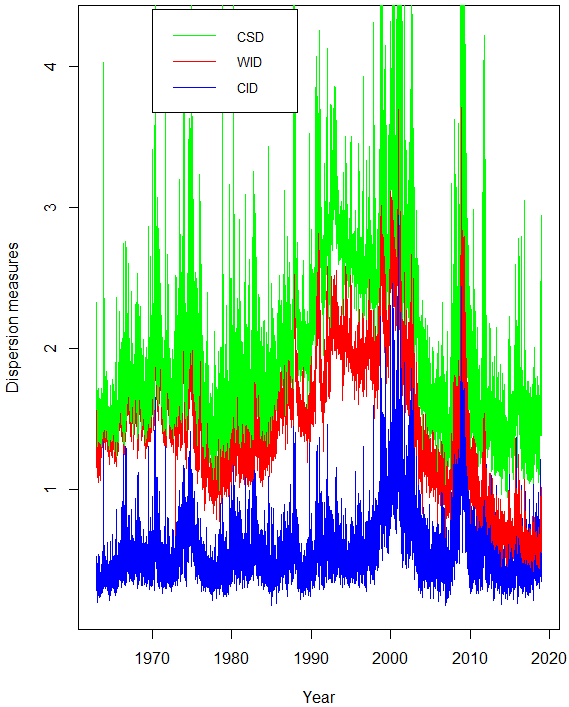
\includegraphics[width=0.9\textwidth]{fig1.png}
\end{figure}

\begin{figure*}
\textbf{Figure 2: Postranking $\beta_{CID}$}
\vskip 12 pt
\begin{flushleft}
{The plot describes the relationship between postranking and preranking $\beta_{CID}$ of decile portfolios, sorted on $\beta_{CID}$.}
\end{flushleft}
\centering
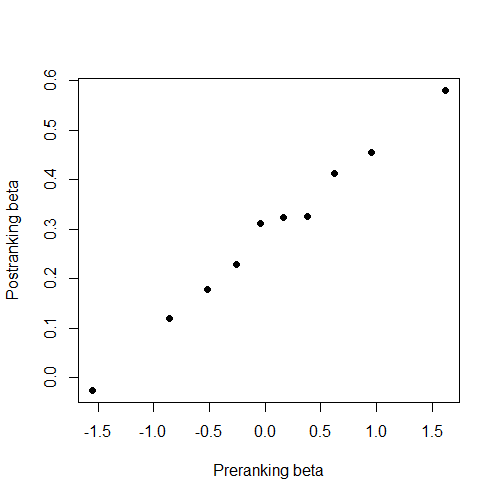
\includegraphics[width=1\textwidth]{Figure2.png}
\end{figure*}


\begin{figure*}
\textbf{Figure 3: Performance of \$1 (log scale)}
\vskip 12 pt
\begin{flushleft}
{The plot describes growth of the investment of \$1 in one of the three portfolios. L/S5 (L/S10) corresponds to long-short portfolio, defined as a difference in returns of extreme quintile (decile) portfolios. Mkt is the value-weighted return of all CRSP stocks(vwretd).}
\end{flushleft}
\centering
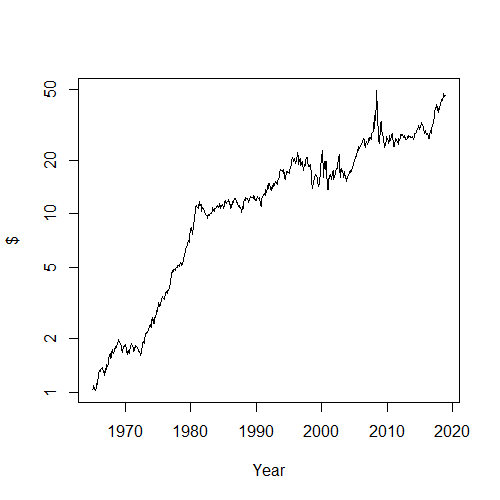
\includegraphics[width=1\textwidth]{Figure3.png}
\end{figure*}


\begin{figure*}
\textbf{Figure 4: Returns of decile L/S portfolio using different Fama-French industry partitions}
\vskip 12 pt
\begin{flushleft}
{The plot describes monthly returns and abnormal returns of decile L/S portfolios, formed on $\beta_{CID}$. I use Fama-French industry definitions with different coarseness: 49, 30, 17, 10 and 5 industries to compute CID. Abnormal returns are calculated with respect to Fama-French 5 factor model, including Momentum and Short-term Reversal factors.}
\end{flushleft}
\centering
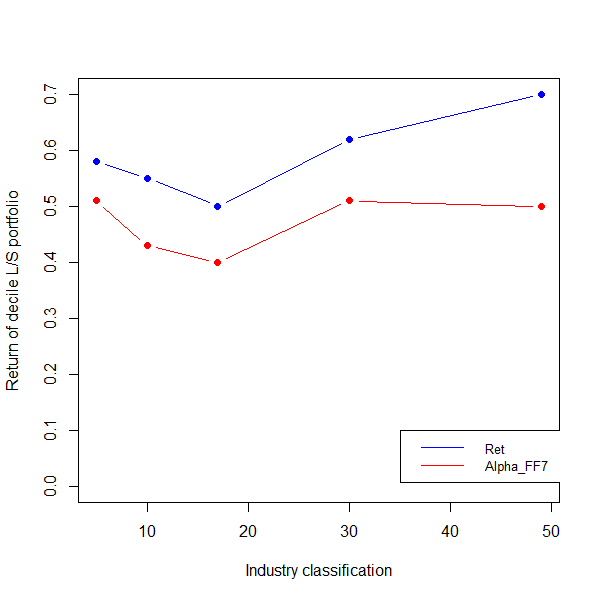
\includegraphics[width=1\textwidth]{alphas_inds.png}
\end{figure*}


\clearpage


% Table created by stargazer v.5.2.2 by Marek Hlavac, Harvard University. E-mail: hlavac at fas.harvard.edu
% Date and time: Tue, Sep 03, 2019 - 1:38:31 PM
\begin{table}[!htbp] \centering 
  \caption{\textbf{Correlations of changes in CID with changes of other variables}} 
  \label{} 
    \begin{flushleft}
    {\medskip\small
 The table reports correlations between changes in CID and changes in other variables at monthly frequency. VIX is implied volatility, available starting from 1990. FU and MU are financial and macroeconomic uncertainty from Sydney Ludvigson website. VOL is the volatility of monthly value-weighted market index over recent 24 months. CIV is common idosyncratic volatility (Kelly et al., 2016). }
    \medskip
    \end{flushleft}
\begin{tabular}{@{\extracolsep{5pt}} ccccccc} 
\\[-1.8ex]\hline 
\hline \\[-1.8ex] 
 & VIX & FU & MU & VOL & CIV & CID \\ 
\hline \\[-1.8ex] 
VIX & $1$ & $0.40$ & $0.36$ & $0.34$ & $0.50$ & $0.12$ \\ 
FU & $0.40$ & $1$ & $0.44$ & $0.30$ & $0.39$ & $0.26$ \\ 
MU & $0.36$ & $0.44$ & $1$ & $0.11$ & $0.24$ & $0.09$ \\ 
VOL & $0.34$ & $0.30$ & $0.11$ & $1$ & $0.27$ & $0.29$ \\ 
CIV & $0.50$ & $0.39$ & $0.24$ & $0.27$ & $1$ & $0.30$ \\ 
CID & $0.12$ & $0.26$ & $0.09$ & $0.29$ & $0.30$ & $1$ \\ 
\hline \\[-1.8ex] 
\end{tabular} 
\end{table}



% Table created by stargazer v.5.2.2 by Marek Hlavac, Harvard University. E-mail: hlavac at fas.harvard.edu
% Date and time: Tue, Sep 03, 2019 - 1:39:07 PM
\begin{table}[!htbp] \centering 
  \caption{\textbf{Characteristics of decile $\beta_{CID}$-sorted vw portfolios}} 
  \label{} 
    \begin{flushleft}
    {\medskip\small
 The table reports mean values of characteristics of decile portfolios, sorted on $\beta_{CID}$. Size is log of market equity in the previous month. bm is log of Book-to-Market. op is operating profitability. BAspr is average bid-ask spread as a percentage of average price over the previous month. }
    \medskip
    \end{flushleft}
\begin{tabular}{@{\extracolsep{0pt}} lccccccccccc} 
\\[-1.8ex]\hline 
\hline \\[-1.8ex] 
 & D1 & D2 & D3 & D4 & D5 & D6 & D7 & D8 & D9 & D10 & LS \\ 
\hline \\[-1.8ex] 
RET & $1.17$ & $0.88$ & $0.86$ & $0.71$ & $0.63$ & $0.65$ & $0.65$ & $0.60$ & $0.52$ & $0.47$ & $$-$0.70$ \\ 
RET\_tstat & $4.80$ & $4.38$ & $4.56$ & $3.97$ & $3.73$ & $3.87$ & $3.69$ & $3.48$ & $2.79$ & $2.12$ & $$-$3.87$ \\ 
preranking beta & $$-$1.55$ & $$-$0.86$ & $$-$0.51$ & $$-$0.26$ & $$-$0.05$ & $0.16$ & $0.38$ & $0.62$ & $0.96$ & $1.62$ & $3.16$ \\ 
postranking beta & $$-$0.03$ & $0.12$ & $0.18$ & $0.23$ & $0.31$ & $0.32$ & $0.33$ & $0.41$ & $0.46$ & $0.58$ & $0.62$ \\ 
size & $7.11$ & $7.71$ & $8.13$ & $8.37$ & $8.60$ & $8.81$ & $8.96$ & $9.16$ & $9.15$ & $8.85$ & $1.74$ \\ 
bm & $6.05$ & $6.12$ & $6.13$ & $6.14$ & $6.14$ & $6.11$ & $6.11$ & $6.07$ & $6.01$ & $5.97$ & $$-$0.08$ \\ 
op & $0.15$ & $0.16$ & $0.17$ & $0.17$ & $0.17$ & $0.17$ & $0.17$ & $0.18$ & $0.18$ & $0.17$ & $0.02$ \\ 
inv & $0.29$ & $0.23$ & $0.18$ & $0.16$ & $0.14$ & $0.13$ & $0.13$ & $0.14$ & $0.14$ & $0.17$ & $$-$0.12$ \\ 
beta & $1.07$ & $0.96$ & $0.91$ & $0.88$ & $0.88$ & $0.89$ & $0.92$ & $0.98$ & $1.08$ & $1.31$ & $0.23$ \\ 
BAspr & $0.39$ & $0.32$ & $0.26$ & $0.24$ & $0.23$ & $0.21$ & $0.20$ & $0.19$ & $0.18$ & $0.18$ & $$-$0.21$ \\ 
mom122 & $0.24$ & $0.18$ & $0.15$ & $0.14$ & $0.12$ & $0.12$ & $0.11$ & $0.11$ & $0.11$ & $0.14$ & $$-$0.10$ \\ 
vol1m & $2.47$ & $2.02$ & $1.82$ & $1.72$ & $1.66$ & $1.61$ & $1.60$ & $1.63$ & $1.74$ & $2.03$ & $$-$0.44$ \\ 
vol12m & $2.63$ & $2.12$ & $1.90$ & $1.79$ & $1.72$ & $1.68$ & $1.67$ & $1.71$ & $1.83$ & $2.19$ & $$-$0.43$ \\ 
\hline \\[-1.8ex] 
\end{tabular} 
\end{table}




% Table created by stargazer v.5.2.2 by Marek Hlavac, Harvard University. E-mail: hlavac at fas.harvard.edu
% Date and time: Tue, Sep 03, 2019 - 2:31:38 PM
\begin{table}[!htbp] \centering 
  \caption{\textbf{Returns of decile $\beta_{CID}$-sorted portfolios}} 
  \label{} 
  \begin{flushleft}
    {\medskip\small
 The table reports mean monthly excess returns of decile portfolios, sorted on $\beta_{CID}$. D1 is the decile portfolio with the lowest $\beta_{CID}$ and D10 contains the highest $\beta_{CID}$ stocks. LS is the long-short portfolio, formed by buying D10 and selling D1. Value-weighted portfolios are constructed by weighting on the market capitalization as of the previous month. The returns are calculated at monthly frequency over 1963-2018.}
    \medskip
    \end{flushleft}
\begin{tabular}{@{\extracolsep{-5pt}} cccccccccccc} 
\\[-1.8ex]\hline 
\hline \\[-1.8ex] 
 & D1 & D2 & D3 & D4 & D5 & D6 & D7 & D8 & D9 & D10 & LS \\ 
\hline \\[-1.8ex] 
Mean ew & 2.50 & 1.79$^{***}$ & 1.58$^{***}$ & 1.41$^{***}$ & 1.36$^{***}$ & 1.32$^{***}$ & 1.29$^{***}$ & 1.26$^{***}$ & 1.29$^{***}$ & 1.61$^{***}$ & -0.89$^{***}$ \\ 
T-stat ew & [9.65] & [8.70] & [8.15] & [7.73] & [7.48] & [7.26] & [6.84] & [6.52] & [6.34] & [6.45] & [-5.72] \\ 
Mean vw & 1.17 & 0.88$^{***}$ & 0.86$^{***}$ & 0.71$^{***}$ & 0.63$^{***}$ & 0.65$^{***}$ & 0.65$^{***}$ & 0.60$^{***}$ & 0.52$^{***}$ & 0.47$^{**}$ & -0.70$^{***}$ \\ 
T-stat vw & [4.80] & [4.38] & [4.56] & [3.97] & [3.73] & [3.87] & [3.69] & [3.48] & [2.79] & [2.12] & [-3.87] \\ 
\hline \\[-1.8ex] 
\end{tabular} 
\end{table}



% Table created by stargazer v.5.2.2 by Marek Hlavac, Harvard University. E-mail: hlavac at fas.harvard.edu
% Date and time: Tue, Sep 03, 2019 - 1:44:52 PM
\begin{table}[!htbp] \centering 
  \caption{\textbf{Abnormal returns of decile $\beta_{CID}$-sorted vw portfolios}} 
  \label{} 
  \begin{flushleft}
    {\medskip\small
 The table reports abnormal monthly returns of long-short value-weighted decile portfolio, formed from sorts on $\beta_{CID}$. The last column contains the abnormal returns with respect to Fama-French 5 factor model, augmented with momentum and short-term reversal factors. The returns are calculated at monthly frequency over 1963-2018.}
    \medskip
    \end{flushleft}
\begin{tabular}{@{\extracolsep{0pt}} ccccccc} 
\\[-1.8ex]\hline 
\hline \\[-1.8ex] 
Statistic & Ret & $\alpha_{CAPM}$ & $\alpha_{FF3}$ & $\alpha_{Carhart}$ & $\alpha_{FF5}$ & $\alpha_{FF5+UMD+STR}$ \\ 
\hline \\[-1.8ex] 
LS & -0.70$^{***}$ & -0.67$^{***}$ & -0.75$^{***}$ & -0.55$^{***}$ & -0.80$^{***}$ & -0.50$^{***}$ \\ 
T-stat & [ -3.87] & [ -3.68] & [ -4.44] & [ -3.24] & [ -4.59] & [ -2.90] \\ 
\hline \\[-1.8ex] 
\end{tabular} 
\end{table}



% Table created by stargazer v.5.2.2 by Marek Hlavac, Harvard University. E-mail: hlavac at fas.harvard.edu
% Date and time: Tue, Sep 03, 2019 - 1:45:59 PM
\begin{table}[!htbp] \centering 
  \caption{\textbf{Factor loadings of decile $\beta_{CID}$-sorted vw portfolios}} 
  \label{} 
  \begin{flushleft}
    {\medskip\small
 The table reports factor loadings of value-weighted portfolios, sorted on $\beta_{CID}$, on Fama-French 5 factor model, augmented with momentum and short-term reversal factors. The returns are calculated at monthly frequency over 1963-2018.}
    \medskip
    \end{flushleft}
\begin{tabular}{@{\extracolsep{0pt}} ccccccccccc} 
\\[-1.8ex]\hline 
\hline \\[-1.8ex] 
Decile & Ret & Alpha & EMKT & HML & SMB & RMW & CMA & Mom & STR & adjR2 \\ 
\hline \\[-1.8ex] 
1 & 1.17 & 0.57 & 1.03 & -0.07 & 0.42 & -0.23 & -0.34 & 0.16 & 0.12 & 0.83 \\ 
 & [ 4.80] & [ 5.24] & [ 38.82] & [ -1.37] & [ 11.75] & [ -4.61] & [ -4.57] & [ 6.39] & [ 3.41] &  \\ 
2 & 0.88 & 0.22 & 0.97 & 0.05 & 0.23 & 0.07 & -0.15 & 0.12 & 0.10 & 0.84 \\ 
 & [ 4.38] & [ 2.46] & [ 45.09] & [ 1.18] & [ 7.84] & [ 1.63] & [ -2.43] & [ 5.67] & [ 3.48] &  \\ 
3 & 0.86 & 0.28 & 0.95 & 0.03 & 0.13 & -0.02 & -0.10 & 0.12 & 0.04 & 0.84 \\ 
 & [ 4.56] & [ 3.40] & [ 47.65] & [ 0.66] & [ 4.98] & [ -0.45] & [ -1.75] & [ 6.48] & [ 1.60] &  \\ 
4 & 0.71 & 0.07 & 0.96 & 0.03 & 0.08 & 0.14 & 0.05 & 0.08 & 0.07 & 0.86 \\ 
 & [ 3.97] & [ 0.92] & [ 54.98] & [ 1.00] & [ 3.56] & [ 4.13] & [ 1.03] & [ 4.67] & [ 2.99] &  \\ 
5 & 0.63 & 0.00 & 0.94 & 0.04 & 0.08 & 0.14 & 0.17 & 0.05 & 0.01 & 0.88 \\ 
 & [ 3.73] & [ -0.02] & [ 60.62] & [ 1.43] & [ 3.60] & [ 4.91] & [ 3.97] & [ 3.37] & [ 0.64] &  \\ 
6 & 0.65 & 0.07 & 0.92 & 0.02 & -0.01 & 0.13 & 0.10 & 0.02 & 0.06 & 0.88 \\ 
 & [ 3.87] & [ 1.20] & [ 60.34] & [ 0.70] & [ -0.27] & [ 4.62] & [ 2.33] & [ 1.38] & [ 3.11] &  \\ 
7 & 0.65 & 0.08 & 0.98 & 0.03 & -0.04 & 0.11 & 0.13 & -0.02 & 0.05 & 0.90 \\ 
 & [ 3.69] & [ 1.36] & [ 67.63] & [ 1.10] & [ -1.81] & [ 3.84] & [ 3.25] & [ -1.65] & [ 2.72] &  \\ 
8 & 0.60 & 0.03 & 1.01 & 0.12 & -0.08 & 0.18 & 0.12 & -0.04 & 0.00 & 0.91 \\ 
 & [ 3.48] & [ 0.47] & [ 74.54] & [ 4.69] & [ -4.30] & [ 7.16] & [ 3.14] & [ -2.98] & [ -0.24] &  \\ 
9 & 0.52 & 0.04 & 1.03 & 0.07 & -0.10 & 0.05 & 0.08 & -0.09 & -0.03 & 0.88 \\ 
 & [ 2.79] & [ 0.60] & [ 60.97] & [ 2.13] & [ -4.17] & [ 1.59] & [ 1.59] & [ -5.27] & [ -1.37] &  \\ 
10 & 0.47 & 0.07 & 1.16 & 0.14 & -0.04 & -0.12 & -0.11 & -0.13 & -0.13 & 0.83 \\ 
 & [ 2.12] & [ 0.71] & [ 47.98] & [ 3.07] & [ -1.15] & [ -2.71] & [ -1.64] & [ -5.54] & [ -3.96] &  \\ 
LS & -0.70 & -0.50 & 0.13 & 0.21 & -0.46 & 0.11 & 0.23 & -0.29 & -0.25 & 0.23 \\ 
 & [ -3.87] & [ -2.90] & [ 3.04] & [ 2.62] & [ -8.05] & [ 1.35] & [ 1.94] & [ -7.20] & [ -4.41] &  \\ 
\hline \\[-1.8ex] 
\end{tabular} 
\end{table} 



% Table created by stargazer v.5.2.2 by Marek Hlavac, Harvard University. E-mail: hlavac at fas.harvard.edu
% Date and time: Tue, Sep 03, 2019 - 1:47:00 PM
\begin{table}[!htbp] \centering 
  \caption{\textbf{Abnormal returns of 2x3 doublesorted portfolios on size and $\beta_{CID}$}}
  \label{} 
  \begin{flushleft}
    {\medskip\small
 The table reports abnormal monthly returns of long-short value-weighted portfolios, formed from independent 2 by 3 double sorts on size and $\beta_{CID}$. By convention, in tercile sort I use 30 and 70 percentiles. The long-short portfolios are formed in the following way:
 $L/S Size = \frac{1}{3}(SmallLow+SmallMedium+SmallHigh) - \frac{1}{3}(BigLow+BigMedium+BigHigh)$,
 $L/S CID = \frac{1}{2}(SmallLow+BigLow) - \frac{1}{2}(SmallHigh+BigHigh)$. \\
 The last column contains the abnormal returns with respect to Fama-French 5 factor model, augmented with momentum and short-term reversal factors. The returns are calculated at monthly frequency over 1963-2018.}
    \medskip
    \end{flushleft}
\begin{tabular}{@{\extracolsep{5pt}} ccccccc} 
\\[-1.8ex]\hline 
\hline \\[-1.8ex] 
Statistic & Ret & $\alpha_{CAPM}$ & $\alpha_{FF3}$ & $\alpha_{Carhart}$ & $\alpha_{FF5}$ & $\alpha_{FF5+UMD+STR}$ \\ 
\hline \\[-1.8ex] 
L/S Size & 0.74$^{***}$ & 0.67$^{***}$ & 0.51$^{***}$ & 0.56$^{***}$ & 0.47$^{***}$ & 0.52$^{***}$ \\ 
T-stat & [ 7.38] & [ 6.84] & [ 12.35] & [ 13.92] & [ 11.30] & [ 12.66] \\ 
L/S CID & 0.22$^{**}$ & 0.23$^{**}$ & 0.28$^{***}$ & 0.15 & 0.31$^{***}$ & 0.16 \\ 
T-stat & [ 2.24] & [ 2.40] & [ 2.91] & [ 1.59] & [ 3.13] & [ 1.61] \\ 
\hline \\[-1.8ex] 
\end{tabular} 
\end{table}



% Table created by stargazer v.5.2.2 by Marek Hlavac, Harvard University. E-mail: hlavac at fas.harvard.edu
% Date and time: Wed, Sep 04, 2019 - 10:02:03 AM
\begin{table}[!htbp] \centering 
  \caption{\textbf{Fama-MacBeth regression}} 
  \label{} 
  \begin{flushleft}
    {\medskip\small
 The table reports the results of Fama-MacBeth regression of excess returns on characteristics of the stocks. Size is log(ME) in the previous month. Momentum is the return over the past year, excluding the most recent month. Investment is defined as the growth in total assets over the recent year. MAX stands for the largest daily return over the previous month. All independent variables are winsorized at 10\% and 90\%. The returns are calculated at monthly frequency over 1963-2018.}
    \medskip
    \end{flushleft}
\begin{tabular}{@{\extracolsep{0pt}}lccccccc} 
\\[-1.8ex]\hline 
\hline \\[-1.8ex] 
 & \multicolumn{7}{c}{\textit{Dependent variable: Return}} \\ 
\cline{2-8} 
\\[-1.8ex] & (1) & (2) & (3) & (4) & (5) & (6) & (7)\\ 
\hline \\[-1.8ex] 
 $\beta_{CID}$ & $-$0.30$^{***}$ & $-$0.31$^{***}$ & $-$0.09$^{**}$ & $-$0.10$^{**}$ & $-$0.09$^{**}$ & $-$0.09$^{***}$ & $-$0.09$^{***}$ \\ 
  & [ $-$4.64] & [ $-$6.50] & [ $-$2.45] & [ $-$2.53] & [ $-$2.39] & [ $-$2.60] & [ $-$2.60] \\ 
  & & & & & & & \\ 
 $\beta_{MKT}$ &  & 0.31 & 0.69$^{***}$ & 0.71$^{***}$ & 0.64$^{***}$ & 0.72$^{***}$ & 0.62$^{***}$ \\ 
  &  & [ 1.54] & [ 3.11] & [ 3.35] & [ 3.17] & [ 3.59] & [ 3.25] \\ 
  & & & & & & & \\ 
 Size &  &  & $-$0.63$^{***}$ & $-$0.62$^{***}$ & $-$0.62$^{***}$ & $-$0.62$^{***}$ & $-$0.58$^{***}$ \\ 
  &  &  & [ $-$14.36] & [ $-$13.63] & [ $-$13.98] & [ $-$14.24] & [ $-$14.57] \\ 
  & & & & & & & \\ 
 Logbm &  &  &  & 0.04 & 0.05 & $-$0.02 & 0.004 \\ 
  &  &  &  & [ 0.77] & [ 0.90] & [ $-$0.28] & [ 0.07] \\ 
  & & & & & & & \\ 
 Momentum &  &  &  &  & 0.04 & 0.01 & 0.02 \\ 
  &  &  &  &  & [ 0.22] & [ 0.04] & [ 0.13] \\ 
  & & & & & & & \\ 
 Investment &  &  &  &  &  & $-$1.23$^{***}$ & $-$1.25$^{***}$ \\ 
  &  &  &  &  &  & [ $-$8.34] & [ $-$8.51] \\ 
  & & & & & & & \\ 
 MAX &  &  &  &  &  &  & 0.02$^{***}$ \\ 
  &  &  &  &  &  &  & [ 3.21] \\ 
  & & & & & & & \\ 
 Constant & 1.49$^{***}$ & 1.21$^{***}$ & 4.58$^{***}$ & 4.51$^{***}$ & 4.49$^{***}$ & 4.56$^{***}$ & 4.26$^{***}$ \\ 
  & [ 7.61] & [ 9.42] & [ 16.03] & [ 15.68] & [ 15.93] & [ 16.38] & [ 16.41] \\ 
  & & & & & & & \\ 
\hline \\[-1.8ex] 
Observations & 1,254,089 & 1,254,089 & 1,254,089 & 1,254,089 & 1,253,020 & 1,226,228 & 1,226,045 \\ 
Adjusted R$^{2}$ & 0.01 & 0.04 & 0.05 & 0.06 & 0.07 & 0.07 & 0.07 \\ 
\hline 
\hline \\[-1.8ex] 
\textit{Note:}  & \multicolumn{7}{r}{$^{*}$p$<$0.1; $^{**}$p$<$0.05; $^{***}$p$<$0.01} \\ 
\end{tabular} 
\end{table}


\clearpage


% Table created by stargazer v.5.2.2 by Marek Hlavac, Harvard University. E-mail: hlavac at fas.harvard.edu
% Date and time: Tue, Sep 03, 2019 - 1:47:48 PM
\begin{table}[!htbp] \centering 
  \caption{\textbf{Abnormal returns of 5x5 doublesorted portfolios on within-industry dispersion $\beta_{WID}$ and $\beta_{CID}$}} 
  \label{} 
  \begin{flushleft}
    {\medskip\small
 The table reports abnormal monthly returns of long-short value-weighted portfolios, formed from independent 5 by 5 double sorts on $\beta_{WID}$ and $\beta_{CID}$. WID (within-industry dispersion) is a mean absolute deviation of returns of the stocks within each industry, averaged across 49 industries. The long-short portfolios are formed in the following way: \\
 $L/S WID = \frac{1}{5}(LowWIDLowCID+LowWIDCID2+LowWIDCID3+LowWIDCID4+LowWIDHighCID) - \frac{1}{5}(HighWIDLowCID+HighWIDCID2+HighWIDCID3+HighWIDCID4+HighWIDHighCID)$, \\
 $L/S CID = \frac{1}{5}(LowCIDLowWID+LowCIDWID2+LowCIDWID3+LowCIDWID4+LowCIDHighWID) - \frac{1}{5}(HighCIDLowWID+HighCIDWID2+HighCIDWID3+HighCIDWID4+HighCIDHighWID)$. \\
 The last column contains the abnormal returns with respect to Fama-French 5 factor model, augmented with momentum and short-term reversal factors. The returns are calculated at monthly frequency over 1963-2018.}
    \medskip
    \end{flushleft}
\begin{tabular}{@{\extracolsep{5pt}} ccccccc} 
\\[-1.8ex]\hline 
\hline \\[-1.8ex] 
Statistic & Ret & $\alpha_{CAPM}$ & $\alpha_{FF3}$ & $\alpha_{Carhart}$ & $\alpha_{FF5}$ & $\alpha_{FF5+UMD+STR}$ \\ 
\hline \\[-1.8ex] 
L/S WID & 0.13 & 0.22 & 0.09 & -0.03 & -0.16 & -0.19 \\ 
T-stat & [ 0.89] & [ 1.46] & [ 0.61] & [ -0.19] & [ -1.08] & [ -1.27] \\ 
L/S CID & 0.38$^{***}$ & 0.34$^{**}$ & 0.44$^{***}$ & 0.38$^{***}$ & 0.59$^{***}$ & 0.43$^{***}$ \\ 
T-stat & [ 2.75] & [ 2.33] & [ 3.16] & [ 2.72] & [ 4.27] & [ 3.06] \\ 
\hline \\[-1.8ex] 
\end{tabular} 
\end{table}



% Table created by stargazer v.5.2.2 by Marek Hlavac, Harvard University. E-mail: hlavac at fas.harvard.edu
% Date and time: Tue, Sep 03, 2019 - 1:48:32 PM
\begin{table}[!htbp] \centering 
  \caption{\textbf{Abnormal returns of 5x5 doublesorted portfolios on cross-sectional dispersion $\beta_{CSD}$ and $\beta_{CID}$}} 
  \label{} 
  \begin{flushleft}
    {\medskip\small
 The table reports abnormal monthly returns of long-short value-weighted portfolios, formed from independent 5 by 5 double sorts on $\beta_{CSD}$ and $\beta_{CID}$. CSD (cross-sectional dispersion) is a mean absolute deviation of returns of all stocks. The long-short portfolios are formed in the following way: \\
$L/S CSD = \frac{1}{5}(LowCSDLowCID+LowCSDCID2+LowCSDCID3+LowCSDCID4+LowCSDHighCID) - \frac{1}{5}(HighCSDLowCID+HighCSDCID2+HighCSDCID3+HighCSDCID4+HighCSDHighCID)$, \\
$L/S CID = \frac{1}{5}(LowCIDLowCSD+LowCIDCSD2+LowCIDCSD3+LowCIDCSD4+LowCIDHighCSD) - \frac{1}{5}(HighCIDLowCSD+HighCIDCSD2+HighCIDCSD3+HighCIDCSD4+HighCIDHighCSD)$. \\
 The last column contains the abnormal returns with respect to Fama-French 5 factor model, augmented with momentum and short-term reversal factors. The returns are calculated at monthly frequency over 1963-2018.}
    \medskip
    \end{flushleft}
\begin{tabular}{@{\extracolsep{5pt}} ccccccc} 
\\[-1.8ex]\hline 
\hline \\[-1.8ex] 
Statistic & Ret & $\alpha_{CAPM}$ & $\alpha_{FF3}$ & $\alpha_{Carhart}$ & $\alpha_{FF5}$ & $\alpha_{FF5+UMD+STR}$ \\  
\hline \\[-1.8ex] 
L/S CSD & -0.03 & 0.07 & -0.03 & -0.15 & -0.21 & -0.32$^{**}$ \\ 
T-stat & [ -0.20] & [ 0.49] & [ -0.24] & [ -1.06] & [ -1.52] & [ -2.24] \\ 
L/S CID & 0.32$^{**}$ & 0.28$^{**}$ & 0.30$^{**}$ & 0.26$^{**}$ & 0.43$^{***}$ & 0.31$^{**}$ \\ 
T-stat & [ 2.46] & [ 2.06] & [ 2.36] & [ 2.00] & [ 3.31] & [ 2.38] \\ 
\hline \\[-1.8ex] 
\end{tabular} 
\end{table}

\begin{table}[!htbp] \centering 
  \caption{\textbf{Abnormal returns of 5x5 doublesorted portfolios on $\beta_{CID}$ and other variables}}
  \label{} 
  \begin{flushleft}
    {\medskip\small
 Construction procedure is equivalent to the one used in the previous tables. CIV is common idiosyncratic volatility from Kelly et al. (2016). MU and FU are macroeconomic and financial uncertainty indices from Ludvigson et al. (2015). Market volatility is a standard deviation of monthly returns over the last 24 months. }
    \medskip
    \end{flushleft}
    
\begin{tabularx}{\linewidth}{p{2cm}p{1.5cm}p{1.5cm}p{1.5cm}p{1.5cm}p{1.5cm}p{1.5cm}}
    \toprule
    \multicolumn{7}{l}{\textbf{Panel A: Market volatility vs CID}} \\
    \midrule 
\\[-1.8ex]\hline 
\hline \\[-1.8ex] 
Statistic & Ret & $\alpha_{CAPM}$ & $\alpha_{FF3}$ & $\alpha_{Carhart}$ & $\alpha_{FF5}$ & $\alpha_{FF5+UMD+STR}$ \\ 
\hline \\[-1.8ex] 
L/S VOL & 0.30$^{**}$ & 0.18 & 0.25$^{**}$ & 0.29$^{**}$ & 0.49$^{***}$ & 0.47$^{***}$ \\ 
T-stat & [ 2.22] & [ 1.36] & [ 1.96] & [ 2.18] & [ 3.85] & [ 3.64] \\ 
L/S CID & 0.40$^{***}$ & 0.42$^{***}$ & 0.45$^{***}$ & 0.32$^{***}$ & 0.48$^{***}$ & 0.30$^{**}$ \\ 
T-stat & [ 3.31] & [ 3.45] & [ 3.84] & [ 2.72] & [ 4.00] & [ 2.48] \\ 
\hline \\[-1.8ex] 
\end{tabularx}



\begin{tabularx}{\linewidth}{p{2cm}p{1.5cm}p{1.5cm}p{1.5cm}p{1.5cm}p{1.5cm}p{1.5cm}}
    \toprule
    \multicolumn{7}{l}{\textbf{Panel B: CIV (Kelly 2016) vs CID}} \\
    \midrule  
\\[-1.8ex]\hline 
\hline \\[-1.8ex] 
Statistic & Ret & $\alpha_{CAPM}$ & $\alpha_{FF3}$ & $\alpha_{Carhart}$ & $\alpha_{FF5}$ & $\alpha_{FF5+UMD+STR}$ \\ 
\hline \\[-1.8ex] 
L/S CIV & 0.33$^{***}$ & 0.27$^{**}$ & 0.16 & 0.21$^{*}$ & 0.08 & 0.13 \\ 
T-stat & [ 2.75] & [ 2.25] & [ 1.41] & [ 1.76] & [ 0.66] & [ 1.04] \\ 
L/S CID & 0.37$^{***}$ & 0.39$^{***}$ & 0.42$^{***}$ & 0.26$^{**}$ & 0.44$^{***}$ & 0.23$^{**}$ \\ 
T-stat & [ 3.06] & [ 3.22] & [ 3.64] & [ 2.27] & [ 3.70] & [ 1.99] \\ 
\hline \\[-1.8ex] 
\end{tabularx} 


\begin{tabularx}{\linewidth}{p{2cm}p{1.5cm}p{1.5cm}p{1.5cm}p{1.5cm}p{1.5cm}p{1.5cm}}
    \toprule
    \multicolumn{7}{l}{\textbf{Panel C: Macroeconomic uncertainty (Ludvigson 2015) vs CID}} \\
    \midrule  
\\[-1.8ex]\hline 
\hline \\[-1.8ex] 
Statistic & Ret & $\alpha_{CAPM}$ & $\alpha_{FF3}$ & $\alpha_{Carhart}$ & $\alpha_{FF5}$ & $\alpha_{FF5+UMD+STR}$ \\ 
\hline \\[-1.8ex] 
L/S MU & 0.05 & -0.07 & -0.03 & 0.08 & 0.19 & 0.19 \\ 
T-stat & [ 0.33] & [ -0.50] & [ -0.20] & [ 0.56] & [ 1.43] & [ 1.44] \\ 
L/S CID & 0.49$^{***}$ & 0.49$^{***}$ & 0.53$^{***}$ & 0.35$^{***}$ & 0.54$^{***}$ & 0.32$^{**}$ \\ 
T-stat & [ 3.76] & [ 3.74] & [ 4.19] & [ 2.82] & [ 4.20] & [ 2.55] \\ 
\hline \\[-1.8ex] 
\end{tabularx} 

\begin{tabularx}{\linewidth}{p{2cm}p{1.5cm}p{1.5cm}p{1.5cm}p{1.5cm}p{1.5cm}p{1.5cm}}
    \toprule
    \multicolumn{7}{l}{\textbf{Panel D: Financial uncertainty (Ludvigson 2015) vs CID}} \\
    \midrule 
\\[-1.8ex]\hline 
\hline \\[-1.8ex] 
Statistic & Ret & $\alpha_{CAPM}$ & $\alpha_{FF3}$ & $\alpha_{Carhart}$ & $\alpha_{FF5}$ & $\alpha_{FF5+UMD+STR}$ \\ 
\hline \\[-1.8ex] 
L/S FU & 0.25$^{*}$ & 0.15 & 0.01 & -0.04 & -0.10 & -0.07 \\ 
T-stat & [ 1.85] & [ 1.14] & [ 0.07] & [ -0.29] & [ -0.79] & [ -0.53] \\ 
L/S CID & 0.39$^{***}$ & 0.40$^{***}$ & 0.44$^{***}$ & 0.31$^{***}$ & 0.45$^{***}$ & 0.28$^{**}$ \\ 
T-stat & [ 3.25] & [ 3.27] & [ 3.75] & [ 2.69] & [ 3.70] & [ 2.33] \\ 
\hline \\[-1.8ex] 
\end{tabularx} 


\begin{tabularx}{\linewidth}{p{2cm}p{1.5cm}p{1.5cm}p{1.5cm}p{1.5cm}p{1.5cm}p{1.5cm}}
    \toprule
    \multicolumn{7}{l}{\textbf{Panel E: VIX vs CID}} \\
    \midrule  
\\[-1.8ex]\hline 
\hline \\[-1.8ex] 
Statistic & Ret & $\alpha_{CAPM}$ & $\alpha_{FF3}$ & $\alpha_{Carhart}$ & $\alpha_{FF5}$ & $\alpha_{FF5+UMD+STR}$ \\ 
\hline \\[-1.8ex] 
L/S VIX & 0.25 & -0.13 & -0.09 & 0.05 & 0.19 & 0.28 \\ 
T-stat & [ 1.08] & [ -0.68] & [ -0.49] & [ 0.30] & [ 1.10] & [ 1.61] \\ 
L/S CID & 0.24 & 0.24 & 0.38$^{**}$ & 0.22 & 0.30 & 0.15 \\ 
T-stat & [ 1.20] & [ 1.19] & [ 2.12] & [ 1.24] & [ 1.64] & [ 0.87] \\ 
\hline \\[-1.8ex] 
\end{tabularx} 

\end{table} 





% Table created by stargazer v.5.2.2 by Marek Hlavac, Harvard University. E-mail: hlavac at fas.harvard.edu
% Date and time: Sun, Sep 08, 2019 - 12:39:04 PM
\begin{table}[!htbp] \centering 
  \caption{\textbf{Predictive regressions for unemployment}}
  \label{} 
      \begin{flushleft}
    {\medskip\small
 The table reports the results of the regression, predicting seasonally-adjusted employment and unemployment at quarterly frequency. Mkt and Vol correspond to value-weighted market return and monthly volatility of value-weighted market returns over most recent 24 months. All dependent variables are differenced using the specification from Pastor and Stambaugh (2003). The sample is restricted to 1948-2019 due to availability of unemployment data.}
    \medskip
    \end{flushleft}
\begin{tabular}{@{\extracolsep{5pt}}lcccc} 
\\[-1.8ex]\hline 
\hline \\[-1.8ex] 
 & \multicolumn{4}{c}{\textit{Dependent variable:}} \\ 
\cline{2-5} 
 & Employment &  & Unemployment &  \\ 
\\[-1.8ex] & (1) & (2) & (3) & (4)\\ 
\hline \\[-1.8ex] 
 CID & $-$0.05$^{**}$ & $-$0.04$^{*}$ & 0.50$^{**}$ & 0.45$^{**}$ \\ 
  & [ $-$2.14] & [ $-$1.80] & [ 2.55] & [ 2.40] \\ 
  & & & & \\ 
 Mkt &  & 0.01$^{**}$ &  & $-$0.23$^{***}$ \\ 
  &  & [ 2.30] &  & [ $-$4.40] \\ 
  & & & & \\ 
 Vol &  & $-$0.003$^{***}$ &  & 0.03$^{***}$ \\ 
  &  & [ $-$2.67] &  & [ 2.79] \\ 
  & & & & \\ 
 Constant & 0.004$^{***}$ & 0.004$^{***}$ & 0.003 & 0.003 \\ 
  & [ 4.71] & [ 5.56] & [ 0.36] & [ 0.41] \\ 
  & & & & \\ 
\hline \\[-1.8ex] 
Observations & 285 & 285 & 283 & 283 \\ 
R$^{2}$ & 0.02 & 0.09 & 0.01 & 0.11 \\ 
Adjusted R$^{2}$ & 0.01 & 0.08 & 0.01 & 0.10 \\ 
\hline 
\hline \\[-1.8ex] 
\textit{Note:}  & \multicolumn{4}{r}{$^{*}$p$<$0.1; $^{**}$p$<$0.05; $^{***}$p$<$0.01} \\ 
\end{tabular} 
\end{table}




\end{document}

